\documentclass[main.tex]{subfiles}
\begin{document}


\section{Теория PQ}\label{ch16}

Большинство квантовых теорий описывают операторы, собственные значения которых образуют континуумы вещественных чисел. Примерами могут служить одна или несколько частиц в некоторой потенциальной яме, гармонические осцилляторы, а также бозонные квантовые поля и струны. Если мы хотим связать их с детерминистическими системами, мы могли бы рассмотреть онтологические наблюдаемые объекты, которые также принимают значения в вещественных числах. Однако есть и другой вариант.

Одним из важных применений преобразований, описанных в этой книге, могут быть наши попытки создать фундаментальные теории о природе в масштабе планка. Здесь мы имеем в действии голографический принцип и предел Бекенштейна $[5] .$ Все это говорит нам о том, что гильбертово пространство, отнесенное к любой малой области пространства, должно быть конечномерным. Напротив, действительные числа описываются неограниченными последовательностями цифр и поэтому требуют бесконечномерных Гильбертовых пространств. Это слишком много. Можно заподозрить, что отношения неопределенности или некоммутативности добавляют к этим числам некоторую размытость. В этой главе мы описываем математическую процедуру для системного подхода.

Для теории $\mathrm{PQ}$, как будет называться наш подход, мы использовали новую нотацию в работах $[114,115],$, где не $\hbar$, а $h$ нормируется на единицу. Тогда волновые функции принимают вид $Е^{2 \pi i p x}=\epsilon^{ipx},$ где $\epsilon=е^{2 i\pi} \approx 535.5$. Эта нотация была очень полезна, чтобы избежать множители $1 / \sqrt{2 \pi}$ для нормализации волновых функций на окружности. Тем не менее мы решили не использовать такую нотацию в этой книге, чтобы избежать столкновений с другими обсуждениями стандартной нотации в различных других главах. Поэтому мы возвращаемся к нормализации $\hbar=1 .$ Множители $\sqrt{2 \pi}$ (для нормализованных состояний) теперь будут встречаться чаще, и, надеюсь, они не будут отпугивать читателя.

В этой главе и части следующих динамические переменные могут быть вещественными числами, обозначенными строчными буквами: $p, q, r, x, \ldots,$ они могут быть целыми числами, обозначенными заглавными буквами: $N, P, Q, X, \ldots,$ или они являются углами (числами, определенными на окружности), обозначенными греческими буквами $\alpha, \eta, \kappa, \varrho, \ldots,$ обычно находящимися в пределах $-\pi<\alpha \leq \pi,$ или иногда определяемыми просто делением с остатком на $2 \pi$.

Действительное число $r$, например число $r=137.035999074\dots,$ состоит из целых, вот так: $R=137,$ и угол $\varrho / 2\pi=0,035999974\dots$. В таких примерах, как квантовая частица на линии, пространство Гильберта простирается в базисе, определенного на линии: $\{|r\rangle\}$. В  $\mathrm{pq}$-теории мы рассматриваем такое пространство Гильберта как произведение пространства Гильберта, охватываемого целыми числами $|R\rangle$ и пространства Гилберта зажатого углами,  $|\varrho\rangle .$ Итак, мы
\begin{equation}\label{16.1}
	\frac{1}{\sqrt{2 \pi}}|r\rangle=|R, \varrho\rangle=|R\rangle|\varrho\rangle
\end{equation}

Обратите внимание, что непрерывность волновой функции $|\psi\rangle$ подразумевает циркулярные граничные условия:

\begin{equation}\label{16.2}
	\langle R+1, \varrho | \psi\rangle=\langle R, \varrho+2 \pi | \psi\rangle
\end{equation}

Дробная часть, или угол, определяется однозначно, но определение интегральной части зависит от того, как угол проецируется на отрезок $[0,2 \pi],$ или: как именно округлить вещественное число до его целочисленного значения? Мы позаботимся об этом, когда столкнемся с проблемой нос к носу.

Пока же мы можем разделить координату $q$ на целое число $Q$ и дробную часть $\xi / 2 \pi$ и ее импульс на целое число $2 \pi P$ и дробную часть $\kappa .$ Теперь мы утверждаем, что это может быть сделано таким образом, что и $[P, Q]=0$ и $[\xi, \kappa]=0$.
Давайте установим нашу алгебру как можно более систематично.



\subsection{Алгебра конечных перестановок}\label{ch16.1}

Введем $q_{\mathrm{op}}$ с невырожденными собственными состояниями $|q\rangle$, имеющими собственные значения $q$, охватывающие всю реальную ось. А также связанный с ним оператор импульса - $p_{\mathrm{op}}$ с собственными функциями $|p\rangle$, тоже с непрерывным спектром. В обычной квантово-механической нотации с $\hbar=1,$ - выходит
\begin{equation}\label{16.3}
q_{\mathrm{op}}|q\rangle= q|q\rangle ; \quad p_{\mathrm{op}}|p\rangle= p|p\rangle ; \quad\left[q_{\mathrm{op}}, p_{\mathrm{op}}\right]=i
\\
\left\langle q | q^{\prime}\right\rangle=\delta\left(q-q^{\prime}\right) ; \quad\left\langle p | p^{\prime}\right\rangle=\delta\left(p-p^{\prime}\right) ; \quad\langle q | p\rangle=\frac{1}{\sqrt{2 \pi}} e^{i p q}
\end{equation}
(часто мы будем опускать подпись 'op', обозначающую, что мы ссылаемся на оператор, если это может  быть понятно из контекста)

Рассмотрим теперь операторы смещения $e^{-i p_{\mathrm{op}} a}$ в пространстве позиций и $e^{i q_{\mathrm{op}} b}$ в пространстве импульсов, где $a$ и $b$ - вещественные числа:

\begin{equation}\label{16.4}
e^{-i p_{\mathrm{op}} a}|q\rangle=|q+a\rangle ; \quad e^{i q_{\mathrm{op}} b}|p\rangle=|p+b\rangle
\end{equation}

имеем

\begin{equation}\label{16.5}
\begin{aligned}
\left[q_{\mathrm{op}}, p_{\mathrm{op}}\right] &=i, \quad e^{i q_{\mathrm{op}} b} p_{\mathrm{op}}=\left(p_{\mathrm{op}}-b\right) e^{i q_{\mathrm{op}} b} \\
e^{i q_{\mathrm{op}} b} e^{-i p_{\mathrm{op}} a} &=e^{-i p_{\mathrm{op}} a} e^{i a b} e^{i q_{\mathrm{op}} b} \\
&=e^{-i p_{\mathrm{op}} a} e^{i q_{\mathrm{op}} b}, \quad \text { if } a b=2 \pi \times \text { integer. }
\end{aligned}
\end{equation}

Рассмотрим оператор смещения в пространстве координат для $a=1 .$ Он унитарен, и поэтому может быть написан однозначно как $e^{-i \kappa},$ где $\kappa$ - эрмитов оператор с собственными значениями $\kappa$, из диапазона $-\pi<\kappa \leq \pi .$ Как видно из ур.\ref{16.4} $\kappa$ также представляет собой результат деления с остатком импульса на $2 \pi .$ Аналогично $e^{i \xi},$ с $-\pi<\xi \leq \pi,$ определяется как оператор, вызывающий сдвиг импульса на шаг $b=2 \pi .$ Это означает, что $\xi / 2 \pi$ - оператор позиции $q$ mod 1. Мы пишем

\begin{equation}\label{16.6}
p=2 \pi K+\kappa, \quad q=X+\xi / 2 \pi
\end{equation}

где и $K$, и $X$ являются целыми числами, а $\kappa$ и $\xi$ - углами. Предлагаем читателю проигнорировать множители $2 \pi$ при первом чтении; они понадобятся только при выполнении точных расчетов.

\subsubsection{От одномерной бесконечной линии до двумерного тора}\label{ch16.1.1}

Как должно быть ясно из ур. (\ref{16.5}) мы можем рассматривать угол $\kappa$ как генератор сдвига в целочисленном $X,$, а угол $\xi$ как генератор сдвига в $K:$

\begin{equation}\label{16.7}
e^{-i \kappa}|X\rangle=|X+1\rangle, \quad e^{i \xi}|K\rangle=|K+1\rangle
\end{equation}

так как $\kappa$ и $\xi$ однозначно определены как генерирующие эти элементарные сдвиги, мы выводим из уравнений (\ref{16.5}) и (\ref{16.7}) что

\begin{equation}\label{16.8}
[\xi, \kappa]=0
\end{equation}

Таким образом, рассмотрим тор, образованный собственными значениями операторов $\kappa$ и $\xi .$ Теперь мы утверждаем, что пространство Гильберта, генерируемое собственными значениями $|\kappa, \xi\rangle$ эквивалентно пространству Гильберта, охваченному собственными значениями $|q\rangle$ оператора $q_{\mathrm{op}},$ или эквивалентно собственным значениям $|p\rangle$ оператора $p_{\mathrm{op}}$ (за исключением ровно одного состояния, см. далее $) $

Сейчас легче всего рассматривать состояния, определенные на этом торе, но мы должны действовать осторожно. Если начать с волновой функции $|\psi\rangle$, которая является непрерывной в $q$, то мы имеем витые периодические граничные условия, как указано в ур.(\ref{16.2}) Запишем в $\xi$ представлении,

\begin{equation}\label{16.9}
\begin{aligned}
\langle X+1, \xi | \psi\rangle &=\langle X, \xi+2 \pi | \psi\rangle, \quad \text { or } \\
\langle\kappa, \xi+ 2 \pi | \psi\rangle &=\left\langle\kappa, \xi\left|e^{i \kappa}\right| \psi\right\rangle
\end{aligned}
\end{equation}

и поскольку эта волновая функция требует, чтоб $X$ был целым, то мы имеем строгую периодичность в $\kappa:$

\begin{equation}\label{16.10}
\langle\kappa+ 2 \pi, \xi | \psi\rangle=\langle\kappa, \xi | \psi\rangle
\end{equation}

Если бы мы рассматривали одно и то же состояние в пространстве импульсов, то периодические граничные условия вели себя по-другому, и поэтому в используемом здесь выражении преобразования из пространства положения в пространство импульсов и обратно являются нетривиальными. Для наших последующих вычислений гораздо лучше сначала перейти к строго периодическому тору. С этой целью мы вводим фазовую функцию $\phi(\kappa, \xi)$ со следующими свойствами:

\begin{equation}\label{16.11}
\phi(\kappa, \xi+2 \pi)=\phi(\kappa, \xi)+\kappa ; \quad \phi(\kappa+2 \pi, \xi)=\phi(\kappa, \xi)
\end{equation}
\begin{equation}\label{16.12}
\phi(\kappa, \xi)=-\phi(-\kappa, \xi)=-\phi(\kappa,-\xi) ; \quad \phi(\kappa, \xi)+\phi(\xi, \kappa)=\kappa \xi / 2 \pi
\end{equation}


Явное выражение для такой функции выведено в \ref{ch16.2} и резюмируется в разделе \ref{ch16.3}. Здесь просто отметим, что эта функция страдает сингулярностью в точке $(\kappa=\pm \pi, \xi=\pm \pi)$. Эта сингулярность является неизбежным следствием требований (\ref{16.11}) и (\ref{16.12}). Это топологический дефект, который можно перемещать по тору, но не утилизировать. Преобразование $|\psi\rangle$ теперь с унитарным преобразованием

\begin{equation}\label{16.13}
\langle\kappa, \xi | \psi\rangle=\langle\kappa, \xi|U(\kappa, \xi)| \tilde{\psi}\rangle ; \quad U(\kappa, \xi)=e^{i \phi(\kappa, \xi)}=e^{i \kappa \xi / 2 \pi-i \phi(\xi, \kappa)}
\end{equation}

превращает граничные условия (\ref{16.9}) и (\ref{16.10}) в строго периодические границы для $|\bar{\psi}\rangle$

Для старой волновой функции мы имели $X=i \partial / \partial \kappa,$, $q_{\mathrm{op}}=i \partial / \partial \kappa+\xi / 2 \pi$. Оператор $p_{\mathrm{op}}$ был бы просто $-2 \pi i \partial / \partial \xi,$ в предположении, что граничное условие (\ref{16.9}) гарантирует, что он сводится к обычному дифференциальному оператору. Наша новая, преобразованная волновая функция теперь требует модификации этих операторов под необычный фазовый множитель $\phi(\kappa, \xi)$. Теперь наши два оператора становятся

\begin{equation}\label{16.14}
q_{\mathrm{op}}=i \frac{\partial}{\partial \kappa}+\frac{\xi}{2 \pi}-\left(\frac{\partial}{\partial \kappa} \phi(\kappa, \xi)\right)=i \frac{\partial}{\partial \kappa}+\left(\frac{\partial}{\partial \kappa} \phi(\xi, \kappa)\right)
\end{equation}

\begin{equation}\label{16.15}
p_{\mathrm{op}}=-2 \pi i \frac{\partial}{\partial \xi}+2 \pi\left(\frac{\partial}{\partial \xi} \phi(\kappa, \xi)\right)=-2 \pi i \frac{\partial}{\partial \xi}+\kappa-2 \pi\left(\frac{\partial}{\partial \xi} \phi(\xi, \kappa)\right)
\end{equation}

Так введение фазового множителя $\phi(\kappa, \xi)$ может восстановить симметрию между операторами $q_{\mathrm{op}}$ и $p_{\mathrm{op}}$. Обратите внимание, что хотя $\phi$ не является периодической, производная $\partial\phi(\kappa,\xi)/\partial\xi$ является и поэтому, $q_{\mathrm{op}}$ и $p_{\mathrm{op}}$ строго периодичны по $\kappa$
и $\xi$ (остерегайтесь отражений $\xi \leftrightarrow \kappa$ в  (\ref{16.14}) и (\ref{16.15}).
Удостоверимся, что они подчиняются правильному коммутационному правилу:

\begin{equation}\label{16.16}
[q_{op},p_{op}] = i
\end{equation}

Очень важно, чтобы эти операторы были периодическими. Это подразумевает, что у нас нет скачков в их определениях. Если бы мы не ввели фазовую функцию $\phi(k, \xi),$ у нас были бы такие тета-скачки, и в таких описаниях матричные элементы в пространстве $Q$, $P$ были бы гораздо менее конвергентным.

Операторы $i \partial / \partial \kappa$ и $-i \partial / \partial \xi$ теперь уже не совсем соответствуют операторам $\mathrm{X}$ и $\mathrm{K}$, из-за последних слагаемых в (\ref{16.14}) и (\ref{16.15}). Они целочисленны и коммутируют, и называть мы их будем $Q$ и $P$. Чтобы получить операторы $q_{\mathrm{op}}$ и $p_{\mathrm{op}}$ в базисе состояний $|Q, P\rangle,$ просто расширим волновые функции в пространстве $\kappa, \xi$ в терминах режимов Фурье,

\begin{equation}\label{16.17}
	\langle\kappa, \xi | Q, P\rangle=\frac{1}{2 \pi} e^{i P \xi-i Q \kappa}
\end{equation}

Теперь нам нужны коэффициенты Фурье фазовой функции $\phi(\kappa, \xi)$. Они приведены в разделе \ref{ch16.2}, где также получены явные выражения для операторов $q_{\mathrm{op}}$ и $p_{\mathrm{op}}$ в базисе $Q, P$:

\begin{equation}\label{16.18} 
\begin{aligned}
q_{\mathrm{op}}=Q_{\mathrm{op}}+a_{\mathrm{op}} ; \quad &\left\langle Q_{1}, P_{1}\left|Q_{\mathrm{op}}\right| Q_{2}, P_{2}\right\rangle= Q_{1} \delta_{Q_{1} Q_{2}} \delta_{P_{1} P_{2}} \\
&\left\langle Q_{1}, P_{1}\left|a_{\mathrm{op}}\right| Q_{2}, P_{2}\right\rangle=\frac{(-1)^{P+Q+1} i P}{2 \pi\left(P^{2}+Q^{2}\right)}
\end{aligned}
\end{equation}

где $Q$ означает $Q_{2}-Q_{1},$ и $P=P_{2}-P_{1}$. Для оператора $p$ аналогично,

\begin{equation}\label{16.19}
p_{\mathrm{op}}=2 \pi P_{\mathrm{op}}+b_{\mathrm{op}}, \quad\left\langle Q_{1}, P_{1}\left|P_{\mathrm{op}}\right| Q_{2}, P_{2}\right\rangle= P_{1} \delta_{Q_{1} Q_{2}} \delta_{P_{1} P_{2}}
\end{equation}

\begin{equation}\label{16.20} 
\left\langle Q_{1}, P_{1}\left|b_{\mathrm{op}}\right| Q_{2}, P_{2}\right\rangle=\frac{(-1)^{P+Q} i Q}{P^{2}+Q^{2}}
\end{equation}

А теперь сюрприз. Рассмотрим коммутатор, [ $\left.q_{\text {op }}, p_{\text {op }}\right]$, в базисе целочисленных $Q$ и $P$. Получим

\begin{equation}\label{16.21} 
\begin{array}{l}
{\left[Q_{\mathrm{op}}, P_{\mathrm{op}}\right]=0 ; \quad\left[a_{\mathrm{op}}, b_{\mathrm{op}}\right]=0} \\
{\left[q_{\mathrm{op}}, p_{\mathrm{op}}\right]=\left[Q_{\mathrm{op}}, b_{\mathrm{op}}\right]+2 \pi\left[a_{\mathrm{op}}, P_{\mathrm{op}}\right]} \\
{\left\langle Q_{1}, P_{1} \| q_{\mathrm{op}}, p_{\mathrm{op}}\right]\left|Q_{2}, P_{2}\right\rangle=- i(-1)^{P+Q}\left(1-\delta Q_{1} Q_{2} \delta P_{1} P_{2}\right)}
\end{array}
\end{equation}

Здесь дельта-функция вставляется потому, что коммутатор исчезает, если $Q_{1}=Q_{2}$ и $P_{1}=P_{2}$. Таким образом, коммутатор не равен $i$ умноженному на чего-нибудь, но может быть записан как

\begin{equation}\label{16.22}
\left[q_{\mathrm{op}}, p_{\mathrm{op}}\right] = i\left(\mathbb{I}-\left|\psi_{e}\right\rangle\left\langle\psi_{e}\right|\right), \quad  \left\langle Q, P | \psi_{e}\right\rangle=(-1)^{P+Q}
\end{equation}

Видимо, есть одно состояние $\left|\psi_{e}\right\rangle$ (с бесконечной нормой), для которого нарушается стандартное правило коммутатора. В этой книге мы сталкиваемся с большим количеством таких состояний, которые можно назвать краевыми состояниями, которые должны быть выведены из нашего пространства Гильберта. С физической точки зрения обычно легко игнорировать краевые состояния, но когда мы делаем математические вычисления, важно понять их природу. Крайнее состояние здесь совпадает с состоянием $\delta(k-\pi) \delta(\xi-\pi),$ поэтому его математическое происхождение легко обнаружить: оно находится в сингулярности нашей вспомогательной фазовой функции $\phi(\kappa, \xi),$, которую мы наблюдали после (\ref{16.11}) и (\ref{16.12}); Видимо, мы должны ограничиться волновыми функциями, которые исчезают в этом месте в $(\kappa, \xi)$ пространстве.

\subsubsection{Состояния $|Q,P\rangle$ в базисе $q$}\label{ch16.1.2}

Как и в других главах, мы хотим идентифицировать матрицу преобразования, позволяющую нам переходить от одной основы к другой. Таким образом, мы хотим найти матричные элементы, связывающие состояния $| Q, P\rangle$ с состояниями $| q\rangle$ или с состояниями $| p\rangle$. Если мы можем найти функцию $\langle q | 0,0\rangle$, которая дает волновую функцию в пространстве $q$ состояния с $Q = P = 0$, то найти остальное будет легко. В разделе $\ref{ch16.4}$ показана производная этой волновой функции. В $(\kappa, \xi)$ пространстве, состояние $|q\rangle$ принимает вид

\begin{equation}\label{16.23} 
\langle\kappa, \xi | q\rangle= e^{i \phi(\kappa, 2 \pi q)} \delta\left(\xi-\xi_{q}\right)
\end{equation}

если $q$ записан как $q=X+\xi_{q} / 2 \pi,$ и $X$ является целым числом. В разделе \ref{ch16.4} показано, что в этом случае волновая функция для $P=Q=0$ равна

\begin{equation}\label{16.24} 
\langle q | 0,0\rangle=\frac{1}{2 \pi} \int_{0}^{2 \pi} \mathrm{d} \kappa e^{-i \phi(\kappa, 2 \pi q)}
\end{equation}

Общая волновая функция получается путем сдвига $P$ и $Q$ на целочисленные суммы:

\begin{equation}\label{16.25} 
\langle q | Q, P\rangle=\frac{1}{2 \pi} e^{2 \pi i P q} \int_{0}^{2 \pi} \mathrm{d} \kappa e^{-i \phi(\kappa, 2 \pi(q-Q))}
\end{equation}

Волновая функция (\ref{16.24}), приравненная к собственному преобразованию Фурье, особенная, так как она близка к блочной волне, имея лишь очень маленькие хвосты вне домена $|q|<\frac{1}{2},$ см. рис. \ref{i16.1}

Волна $\langle q | Q, P\rangle$ аналогична так называемым вейвлетам $[83],$, которые иногда используются для описания импульсных волн, но у этой волны есть два дополнительных признака. Она не только равно своему собственному преобразованию Фурье, но и ортогонально сама себе при сдвиге на целое число. Это делает набор волн $|Q, P\rangle$ в (\ref{16.25}) ортонормированным базисом. Этот $P Q$ формализм предназначен для преобразования систем, основанных только на целочисленных числах, в системы, основанные на вещественных числах, и обратно. Можно предположить, что целые числа подвергаются переключениям, описываемым оператором перестановки $\mathcal{P}_{\mathrm{op}}$. После определения некоторого полезного выражения для гамильтониана $H_{\mathrm{op}}$, с $\mathcal{P}_{\mathrm{op}}=e^{-i \hat{H}_{\mathrm{op}} \delta t}$, можно преобразовать это дело в квантовую систему с этим гамильтонианом в ее новом базисе. 

Для одной пары $P Q$ построить детерминистическую модель, оператор эволюции которой напоминает реалистичный квантовый гамильтониан, сложно. Точный, канонический, дискретный гамильтоновский формализм возможен в схеме $P Q$, но он требует некоторой дополнительной работы, которую мы откладываем до секции \ref{ch19}. Интересные гамильтонианцы получены в многомерном случае: $P_{i}, Q_{i} .$ Такая система рассматривается в главе \ref{ch17}.
 
\begin{figure}[ht]
	\begin{center}
		\scalebox{0.4}{
		   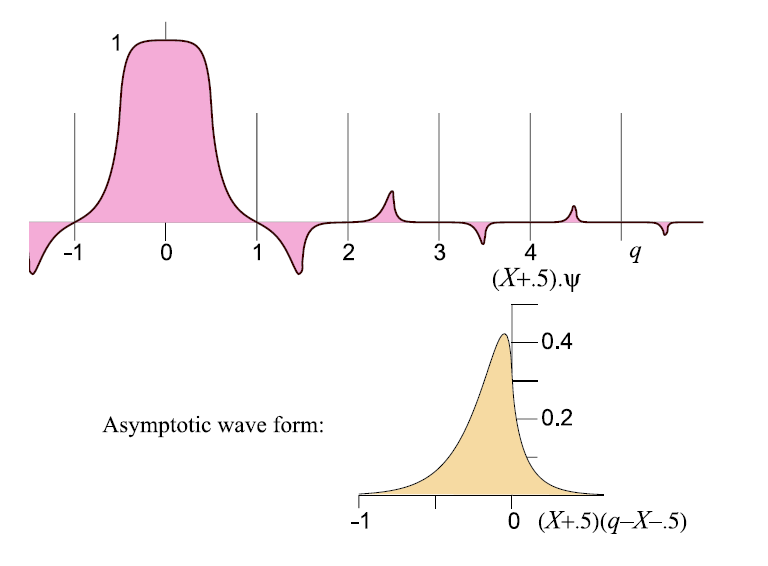
\includegraphics{images/img_16_1.png}
		}
		\caption{
		\label{i16.1} Волновая функция состояния $|Q, P\rangle$ при $P =Q= 0$. Ниже асимптотическая форма отмасштабированных маленьких пиков, удаленных от центра}
	\end {center}
\end {figure}



\subsection{Преобразования в PQ-формализме}\label{ch16.2}

Следующие разделы можно читать как Приложения к части 16. Они содержат технические особенности, которые могут быть неинтересны большинству читателей, но они необходимы для понимания нюансов, с которыми пришлось столкнуться, в частности, когда проводились явные вычисления, соединяющие базовые наборы вещественных чисел $q$, их Фурье преобразование $p$, целые $(Q, P)$ и тор $(\kappa, \xi)$.

Сначала построим решение граничных условий (\ref{16.11}) и (\ref{16.12}) для фазовой функции $\phi(\kappa, \xi)$

\begin{equation}\label{16.26} 
\begin{array}{l}
{\phi(\kappa, \xi+2 \pi)=\phi(\kappa, \xi)+\kappa ; \quad \phi(\kappa+2 \pi, \xi)=\phi(\kappa, \xi)} \\
{\phi(\kappa, \xi)=-\phi(-\kappa, \xi)=-\phi(\kappa,-\xi) ; \quad \phi(\kappa, \xi)+\phi(\xi, \kappa)=\kappa \xi / 2 \pi}
\end{array}
\end{equation}

На первый взгляд, эти условия кажутся противоречивыми. Если мы следуем закрытому контуру $(\kappa, \xi)=(0,0) \rightarrow(2 \pi, 0) \rightarrow(2 \pi, 2 \pi) \rightarrow(0,2 \pi) \rightarrow(0,0),$, то подбираем слагаемое $2 \pi .$ Это означает, что функции, которая везде имеет единое значение, не существует, следовательно, у нас должна быть сингулярность. Можно записать амплитуду $\psi(\kappa, \xi)=r e^{i \phi}$ для которой наша фи будет фазой, но эта функция должна иметь ноль или полюс. Предположим, что она имеет ноль, а $r$ просто периодична. Тогда можно найти самое гладкое решение. Если $r$ и $\phi$ - это реальные функции:
$r$

\begin{equation}\label{16.28} 
r(\kappa, \xi) e^{i \phi(\kappa, \xi)}=\sum_{N=-\infty}^{\infty} e^{-\pi\left(N-\frac{\xi}{2 \pi}\right)^{2}+i N \kappa}
\end{equation}

можно обнаружить периодичность в $\kappa$, в то время как замена

\begin{equation}\label{16.29} 
\xi \rightarrow \xi+2 \pi, \quad N \rightarrow N+1
\end{equation}

дает первую часть (\ref{16.26}). Сумма в (\ref{16.28}), которая, к счастью, быстро сходится, является особым случаем эллиптической функции $\vartheta_{3},$ и ее также можно записать как произведение $[31,45]:$

\begin{equation}\label{16.30} 
\begin{aligned}
r(\kappa, \xi) e^{i \phi(\kappa, \xi)}=& e^{-\frac{\xi^{2}}{4 \pi}} \prod_{N=1}^{\infty}\left(1-e^{-2 \pi N}\right) \\
\times \prod_{N=0}^{\infty}\left(1+e^{\xi+i \kappa-2 \pi N-\pi}\right)\left(1+e^{-\xi-i \kappa-2 \pi N-\pi}\right) &
\end{aligned}
\end{equation}

из чего мы можем легко считывать нули: они находятся по адресу $(\kappa, \xi)=\left(2 \pi N_{1}+\pi\right.$ $2 \pi N_{2}+\pi$ ). Мы сознательно выбрали их так, чтобы они находились на углах $(\pm \pi, \pm \pi)$ тора, но на самом деле не имеет значения, где они находятся; они просто неизбежны.

Матричные элементы $\left\langle Q_{1}, P_{1}\left|q_{\mathrm{op}}\right| Q_{2}, P_{2}\right\rangle$ получают путем их первого вычисления на торе. Таким образом\footnote{Приносим извинения за то, что в некоторых местах переменные $\kappa$ и $\xi$ поменялись, что было неизбежно, пожалуйста, будьте внимательны.}

\begin{equation}\label{16.} 
q_{\mathrm{op}}=Q_{\mathrm{op}}+a(\xi, \kappa) ; \quad Q_{\mathrm{op}}=i \frac{\partial}{\partial \kappa}, \quad a(\xi, \kappa)=\left(\frac{\partial}{\partial \kappa} \phi(\xi, \kappa)\right)
\end{equation}


Для расчета $a(\xi, \kappa)$ сгодится (\ref{16.30}):

\begin{equation}\label{16.32} 
\begin{aligned}
a(\xi, \kappa) &=\sum_{N=0}^{\infty} a_{N}(\xi, \kappa) \\
a_{N}(\xi, \kappa) &=\frac{\partial}{\partial \kappa}\left(\arg \left(1+e^{\kappa+i \xi-2 \pi\left(N+\frac{1}{2}\right)}\right)+\arg \left(1+e^{-\kappa-i \xi-2 \pi\left(N+\frac{1}{2}\right)}\right)\right)
\end{aligned}
\end{equation}

Оценка дает (обратите внимание на обмен $\kappa$ и $\xi$ ):

\begin{equation}\label{16.33}
a_{N}(\xi, \kappa)=\frac{\frac{1}{2} \sin \xi}{\cos \xi+\cosh (\kappa-2 \pi N-\pi)}+\frac{\frac{1}{2} \sin \xi}{\cos \xi+\cosh (\kappa+2 \pi N+\pi)}
\end{equation}

что теперь позволяет нам переписать его как одну сумму по $N$, которая будет от $-\infty$ до $\infty$ вместо от нуля до $\infty$.

Сначала преобразовываем из базиса $\xi$ в $P$, оставляя $\kappa$ без изменений. Это превращает $a(\xi, \kappa)$ в оператор $a_{\mathrm{op}}$. Используя

\begin{equation}\label{16.34} 
\left\langle P_{1} | \xi\right\rangle\left\langle\xi | P_{2}\right\rangle=\frac{1}{2 \pi} e^{i P \xi}, \quad P=P_{2}-P_{1}
\end{equation}

мы получим матричный элемент оператора $a_{\mathrm{op}}$ в представлении $(P, \kappa)$:

\begin{equation}\label{16.35} 
\left\langle P_{1}\left|a_{\mathrm{op}}(\kappa)\right| P_{2}\right\rangle=\sum_{N=-\infty}^{\infty} a_{N}(P, \kappa), \quad P \equiv P_{2}-P_{1}
\end{equation}

и записав $z=e^{i \xi},$ находим

\begin{equation}\label{16.36}
\begin{array}{l}
a_{N}(P, \kappa)=\oint \frac{\mathrm{d} z}{2 \pi i z} z^{P} \frac{-\frac{1}{2} i(z-1 / z)}{z+1 / z+e^{R}+e^{-R}}, \quad R=\kappa+2 \pi N+\pi \\
a_{N}(P, \kappa)=\frac{1}{2} \operatorname{sgn}(P)(-1)^{P-1} i e^{-|P(\kappa+2 \pi N+\pi)|}
\end{array}
\end{equation}

где $\operatorname{sgn}(P)$ определен как $\pm 1$ если $P \geq 0$ и 0 если $P=0 .$ Абсолютное значение, взятое в экспоненте, действительно означает, что там всегда есть отрицательный аргумент; оно возникло, когда контур, интеграл по единичной окружности, заставил нас выбрать полюс внутри единичной окружности.

Затем, находим $(Q, P)$ матричные элементы взаимодействуя через $\kappa$ с множителем $\left\langle Q_{1} | \kappa\right\rangle\left\langle\kappa | Q_{2}\right\rangle=\frac{1}{2 \pi} e^{i Q \kappa},$ with $Q=Q_{2}-Q_{1} .$ Сумируя по $N$ и интегрмруя по $\kappa$ от 0 до $2 \pi$ combine integral over all real values of $\kappa,$ получим удивительно простое выражение

\begin{equation}\label{16.37} 
\left\langle Q_{1}, P_{1}\left|a_{\mathrm{op}}\right| Q_{2}, P_{2}\right\rangle=\frac{(-1)^{P+Q+1} i P}{2 \pi\left(P^{2}+Q^{2}\right)}
\end{equation}

В (\ref{16.14}), оно дает для оператора $q$:

\begin{equation}\label{16.38}
	\begin{array}{c}
{q_{\mathrm{op}}=Q_{\mathrm{op}}+a_{\mathrm{op}}} \\
{\left\langle Q_{1}, P_{1}\left|q_{\mathrm{op}}\right| Q_{2}, P_{2}\right\rangle= Q_{1} \delta_{Q_{1} Q_{2}} \delta_{P_{1} P_{2}}+\left\langle Q_{1}, P_{1}\left|a_{\mathrm{op}}\right| Q_{2}, P_{2}\right\rangle}
\end{array}
\end{equation}

А для $p$ используем (\ref{16.31})

\begin{equation}\label{16.39}
	p_{\mathrm{op}}=2 \pi P+b(\kappa, \xi) ; \quad P=-i \frac{\partial}{\partial \xi}, \quad b(\kappa, \xi)=2 \pi\left(\frac{\partial}{\partial \xi} \phi(\kappa, \xi)\right)
\end{equation}

не забыв про $P \equiv P_2 − P_1$,

\begin{equation}\label{16.40}
	\begin{aligned}
&p_{\mathrm{op}}=2 \pi P_{\mathrm{op}}+b_{\mathrm{op}}, \quad\left\langle Q_{1}, P_{1}\left|P_{\mathrm{op}}\right| Q_{2}, P_{2}\right\rangle= P_{1} \delta_{Q_{1} Q_{2}} \delta_{P_{1} P_{2}}\\
&\left\langle Q_{1}, P_{1}\left|b_{\mathrm{op}}\right| Q_{2}, P_{2}\right\rangle=\frac{(-1)^{P+Q} i Q}{P^{2}+Q^{2}}
\end{aligned}
\end{equation}

Обратите внимание, во всех этих выражениях мы имеем симметрию под комбинированным обменом

\begin{equation}\label{16.42}
	\begin{aligned}
&p_{\mathrm{op}} \leftrightarrow 2 \pi q_{\mathrm{op}}, \quad P \leftrightarrow Q, \quad X \leftrightarrow K\\
&\xi \leftrightarrow \kappa, \quad i \leftrightarrow-i, \quad 2 \pi a_{\mathrm{op}} \leftrightarrow b_{\mathrm{op}}
\end{aligned}
\end{equation}





\subsection{Резюме для квазипериодической фазовой функции $\phi(\xi, \kappa)$}\label{ch16.3}

Положим $Q$ и $P$ целочисленные, а $\xi$ и $\kappa$ подчиняются $-\pi<\xi<\pi,-\pi<\kappa<\pi$. Эти операторы подчиняются
\begin{equation}\label{16.} 
\left[Q_{\mathrm{op}}, P_{\mathrm{op}}\right]=\left[\xi_{\mathrm{op}}, P_{\mathrm{op}}\right]=\left[Q_{\mathrm{op}}, \kappa_{\mathrm{op}}\right]=\left[\xi_{\mathrm{op}}, \kappa_{\mathrm{op}}\right]=0
\end{equation}

Скалярные произведения:

\begin{equation}\label{16.44}
\langle\kappa | Q\rangle=\frac{1}{\sqrt{2 \pi}} e^{-i Q \kappa}\quad
\langle\xi | P\rangle=\frac{1}{\sqrt{2 \pi}} e^{i P \xi}
\end{equation}

Функции фазового угла $\phi$ и $\tilde{\phi}$ определены как подчиняющиеся (\ref{16.26}) и (\ref{16.27}) и

\begin{equation}\label{16.45} 
\tilde{\phi}(\xi, \kappa)=\phi(\kappa, \xi), \quad \phi(\xi, \kappa)+\tilde{\phi}(\xi, \kappa)=\xi \kappa / 2 \pi
\end{equation}

При вычислении матричных элементов не следует брать сам оператор $\phi$, так как он является псевдо-периодическим, а не периодическим, так что краевое состояние $\delta(\kappa \pm \pi)$ дает сингулярности. А вот оператор $\partial \phi(\xi, \kappa) / \partial \kappa \equiv a(\xi, \kappa)$ является периодическим, поэтому мы начинаем с него. Обратите внимание, что на $(\xi, \kappa)$-торе наши вычисления часто заставляют нас менять порядок следования переменных $\xi$ и $\kappa .$ Таким образом, в слегка измененной нотации,

\begin{equation}\label{16.46}
	a(\xi, \kappa)=\sum_{N=-\infty}^{\infty} a_{N}(\xi, \kappa) ; \quad a_{N}(\xi, \kappa)=\frac{\frac{1}{2} \sin \xi}{\cos \xi+\cosh \left(\kappa+2 \pi\left(N+\frac{1}{2}\right)\right)}
\end{equation}

вспоминая что $P_{2}-P_{1} \equiv P,$ запишем в $(\kappa, P)$-базисе

\begin{equation}\label{16.47} 
\begin{array}{l}
{\left\langle\kappa_{1}, P_{1}\left|a_{N}^{\mathrm{op}}\right| \kappa_{2}, P_{2}\right\rangle=\delta\left(\kappa_{1}-\kappa_{2}\right) a_{N}\left(\kappa_{1}, P\right)} \\
{a_{N}(\kappa, P) \equiv \frac{1}{2 \pi} \int_{0}^{2 \pi} \mathrm{d} \xi e^{i P \xi} a_{N}(\xi, \kappa)=\frac{1}{2} \operatorname{sgn}(P)(-1)^{P-1} i e^{-|P(\kappa+2 \pi N+\pi)|}} \\
{a(\kappa, P)=\frac{1}{2} i(-1)^{P-1} \frac{\cosh (P \kappa)}{\sinh (P \pi)}}
\end{array}
\end{equation}

И наоборот, мы можем получить в $(Q, \xi)$ базисе, используя $Q_{2}-Q_{1}=Q:$ 

\begin{equation}
\left\langle Q_{1}, \xi_{1}\left|a_{N}^{\mathrm{op}}\right| Q_{2}, \xi_{2}\right\rangle=\delta\left(\xi_{1}-\xi_{2}\right) a_{N}\left(Q, \xi_{1}\right)
\end{equation}

\begin{equation}\label{16.48} 
\begin{aligned}
a_{N}(Q, \xi) &=\frac{1}{4 \pi} \sin \xi \int_{-\pi}^{\pi} \mathrm{d} \kappa \frac{e^{i Q_{k}}}{\cos \xi+\cosh (\kappa+2 \pi N+\pi)} \\
a(Q, \xi) &=\sum_{N} a_{N}(Q, \xi)=(-1)^{Q} \frac{\sinh (Q \xi)}{2 \sinh (Q \pi)}
\end{aligned}
\end{equation}

(последнее выражение встречается при интегрировании контуров). Наконец, в $(Q, P)$-базисе, мы имеем, либо по преобразованию Фурье (\ref{16.47}), либо по преобразованию (\ref{16.48}):

\begin{equation}\label{16.49} 
\left\langle Q_{1}, P_{1}\left|a^{\mathrm{op}}\right| Q_{2}, P_{2}\right\rangle=\frac{-i}{2 \pi}(-1)^{Q+P} \frac{P}{Q^{2}+P^{2}}
\end{equation}

Операторы $q_{\mathrm{op}}$ и $p_{\mathrm{op}}$ теперь определены на торе как

\begin{equation}\label{16.50} 
q_{\mathrm{op}}(\kappa, \xi)=Q_{\mathrm{op}}+a(\xi, \kappa), \quad p_{\mathrm{op}}(\kappa, \xi)=2 \pi\left(P_{\mathrm{op}}+a(\kappa, \xi)\right)
\end{equation}

и $Q_{\mathrm{op}}=i \partial / \partial \kappa, P_{\mathrm{op}}=-i \partial / \partial \xi .$ Отсюда выходят уравнения (\ref{16.37}) и (\ref{16.41})



\subsection{Волновая функция состояния $|0, 0\rangle$}\label{ch16.4}

Расчитаем состояние $|q\rangle$ на $(\kappa, \xi)$ торе. Его волновая функция (смотри (\ref{16.14}))

\begin{equation}\label{16.51} 
q_{\mathrm{op}}|q\rangle= i e^{i \phi(\xi, \kappa)} \frac{\partial}{\partial \kappa}\left(e^{-i \phi(\xi, \kappa)}|q\rangle\right)=q|q\rangle
\end{equation}

Это уравнение легко решить:

\begin{equation}\label{16.52} 
\langle\kappa, \xi | q\rangle= C(\xi) e^{i \phi(\xi, \kappa)-i q \kappa}
\end{equation}

Поскольку решение должно быть периодическим по $\kappa$ и $\xi$, то, хотя у нас есть условия периодичности (\ref{16.26}) для $\phi,$, мы выводим, что решение есть только в том случае, если $\xi / 2 \pi$ является дробной частью $q$ или $q=X+\xi / 2 \pi$, где $X$ - целое число. В таком случае, мы можем написать

\begin{equation}\label{16.53} 
\langle\kappa, \xi | q\rangle= C(\xi) e^{-i X \kappa-i \phi(\kappa, \xi)}=C(\xi) e^{-i \phi(\kappa, 2 \pi q)}
\end{equation}

Таким образом, полный матричный элемент, при $q=X+\xi_{q} / 2 \pi$ имеет вид

\begin{equation}\label{16.54} 
\langle\kappa, \xi | q\rangle= C e^{-i \phi(\kappa, 2 \pi q)} \delta\left(\xi-\xi_{q}\right)
\end{equation}

(обратите внимание, что фаза $\phi(\kappa, \xi)$ не является периодической во второй записи $\xi$; записи обратны по сравнению с (\ref{16.26})). Нормализация вытекает из требования

\begin{equation}\label{16.55}
	\begin{aligned}
\int_{0}^{2 \pi} \mathrm{d} \kappa \int_{0}^{2 \pi} \mathrm{d} \xi\left\langle q_{1} | \kappa, \xi\right\rangle\left\langle\kappa, \xi | q_{2}\right\rangle &=\delta\left(q_{1}-q_{2}\right) \\
\int_{-\infty}^{\infty} \mathrm{d} q\left\langle\kappa_{1}, \xi_{1} | q\right\rangle\left\langle q | \kappa_{2}, \xi_{2}\right\rangle &=\delta\left(\kappa_{1}-\kappa_{2}\right) \delta\left(\xi_{1}-\xi_{2}\right)
\end{aligned}
\end{equation}

из которого

\begin{equation}\label{16.56}
	C=1
\end{equation}

Обратите внимание, что мы выбрали фазу +1. Как и в других местах этой книги, фазы могут быть выбраны свободно.

Из

\begin{equation}\label{16.57}
	\langle\kappa, \xi | Q, P\rangle=\frac{1}{2 \pi} e^{i P \xi-i Q \kappa}
\end{equation}

получим

\begin{equation}\label{16.58}
	\begin{aligned}
\langle q | Q, P\rangle &=\frac{1}{2 \pi} \int_{0}^{2 \pi} \mathrm{d} \kappa e^{i P \xi-i Q \kappa+i \phi(\kappa, 2 \pi q)} \\
&=\frac{1}{2 \pi} e^{2 \pi i P q} \int_{0}^{2 \pi} \mathrm{d} \kappa e^{i \phi(\kappa, 2 \pi(q-Q))}
\end{aligned}
\end{equation}






\if 0

\begin{equation}\label{16.3}
	\begin{array}{l}
{q_{\mathrm{op}}|q\rangle= q|q\rangle ; \quad p_{\mathrm{op}}|p\rangle= p|p\rangle ; \quad\left[q_{\mathrm{op}}, p_{\mathrm{op}}\right]=i} \\
{\left\langle q | q^{\prime}\right\rangle=\delta\left(q-q^{\prime}\right) ; \quad\left\langle p | p^{\prime}\right\rangle=\delta\left(p-p^{\prime}\right) ; \quad\langle q | p\rangle=\frac{1}{\sqrt{2 \pi}} e^{i p q}}
\end{array}
\end{equation}

\begin{equation}\label{16.4}
	e^{-i p_{\mathrm{op}} a}|q\rangle=|q+a\rangle ; \quad e^{i q_{\mathrm{op}} b}|p\rangle=|p+b\rangle
\end{equation}

\begin{equation}\label{16.5}
	\begin{aligned}
\left[q_{\mathrm{op}}, p_{\mathrm{op}}\right] &=i, \quad e^{i q_{\mathrm{op}} b} p_{\mathrm{op}}=\left(p_{\mathrm{op}}-b\right) e^{i q_{\mathrm{op}} b} \\
e^{i q_{\mathrm{op}} b} e^{-i p_{\mathrm{op}} a} &=e^{-i p_{\mathrm{op}} a} e^{i a b} e^{i q_{\mathrm{op}} b} \\
&=e^{-i p_{\mathrm{op}} a} e^{i q_{\mathrm{op}} b}, \quad \text { if } a b=2 \pi \times \text { integer }
\end{aligned}
\end{equation}

\begin{equation}\label{16.6}
	p=2 \pi K+\kappa, \quad q=X+\xi / 2 \pi
\end{equation}

\begin{equation}\label{16.7}
	e^{-i \kappa}|X\rangle=|X+1\rangle, \quad e^{i \xi}|K\rangle=|K+1\rangle
\end{equation}

\begin{equation}\label{16.8}
	[\xi,k] = 0
\end{equation}

\begin{equation}\label{16.9}
	\begin{aligned}
\langle X+1, \xi | \psi\rangle &=\langle X, \xi+2 \pi | \psi\rangle \\
\langle\kappa, \xi+ 2 \pi | \psi\rangle &=\left\langle\kappa, \xi\left|e^{i \kappa}\right| \psi\right\rangle
\end{aligned}
\end{equation}

\begin{equation}\label{16.10}
	\langle\kappa+ 2 \pi, \xi | \psi\rangle=\langle\kappa, \xi | \psi\rangle
\end{equation}

\begin{equation}\label{16.11}
	\begin{aligned}
&\phi(\kappa, \xi+2 \pi)=\phi(\kappa, \xi)+\kappa ; \quad \phi(\kappa+2 \pi, \xi)=\phi(\kappa, \xi)\\
&\phi(\kappa, \xi)=-\phi(-\kappa, \xi)=-\phi(\kappa,-\xi) ; \quad \phi(\kappa, \xi)+\phi(\xi, \kappa)=\kappa \xi / 2 \pi
\end{aligned}
\end{equation}

\begin{equation}\label{16.13}
	\langle\kappa, \xi | \psi\rangle=\langle\kappa, \xi|U(\kappa, \xi)| \tilde{\psi}\rangle ; \quad U(\kappa, \xi)=e^{i \phi(\kappa, \xi)}=e^{i \kappa \xi / 2 \pi-i \phi(\xi, \kappa)}
\end{equation}

\begin{equation}\label{16.14}
	\begin{aligned}
&q_{\mathrm{op}}=i \frac{\partial}{\partial \kappa}+\frac{\xi}{2 \pi}-\left(\frac{\partial}{\partial \kappa} \phi(\kappa, \xi)\right)=i \frac{\partial}{\partial \kappa}+\left(\frac{\partial}{\partial \kappa} \phi(\xi, \kappa)\right)\\
&p_{\mathrm{op}}=-2 \pi i \frac{\partial}{\partial \xi}+2 \pi\left(\frac{\partial}{\partial \xi} \phi(\kappa, \xi)\right)=-2 \pi i \frac{\partial}{\partial \xi}+\kappa-2 \pi\left(\frac{\partial}{\partial \xi} \phi(\xi, \kappa)\right)
\end{aligned}
\end{equation}

\begin{equation}\label{16.16}
	[\hat q, \hat p] = i
\end{equation}



\begin{equation}\label{16.18}
	\begin{aligned}
q_{\mathrm{op}}=Q_{\mathrm{op}}+a_{\mathrm{op}} ; \quad &\left\langle Q_{1}, P_{1}\left|Q_{\mathrm{op}}\right| Q_{2}, P_{2}\right\rangle= Q_{1} \delta_{Q_{1} Q_{2}} \delta_{P_{1} P_{2}} \\
&\left\langle Q_{1}, P_{1}\left|a_{\mathrm{op}}\right| Q_{2}, P_{2}\right\rangle=\frac{(-1)^{P+Q+1} i P}{2 \pi\left(P^{2}+Q^{2}\right)}
\end{aligned}
\end{equation}



\begin{equation}\label{16.19}
	\begin{aligned}
&p_{\mathrm{op}}=2 \pi P_{\mathrm{op}}+b_{\mathrm{op}}, \quad\left\langle Q_{1}, P_{1}\left|P_{\mathrm{op}}\right| Q_{2}, P_{2}\right\rangle= P_{1} \delta_{Q_{1} Q_{2}} \delta_{P_{1} P_{2}}\\
&\left\langle Q_{1}, P_{1}\left|b_{\mathrm{op}}\right| Q_{2}, P_{2}\right\rangle=\frac{(-1)^{P+Q} i Q}{P^{2}+Q^{2}}
\end{aligned}
\end{equation}



\begin{equation}\label{16.21}
	\begin{aligned}
&\left[Q_{\mathrm{op}}, P_{\mathrm{op}}\right]=0 ; \quad\left[a_{\mathrm{op}}, b_{\mathrm{op}}\right]=0\\
&\left[q_{\mathrm{op}}, p_{\mathrm{op}}\right]=\left[Q_{\mathrm{op}}, b_{\mathrm{op}}\right]+2 \pi\left[a_{\mathrm{op}}, P_{\mathrm{op}}\right]\\
&\left\langle Q_{1}, P_{1}\left|\left[q_{\mathrm{op}}, p_{\mathrm{op}}\right]\right| Q_{2}, P_{2}\right\rangle=- i(-1)^{P+Q}\left(1-\delta_{Q_{1} Q_{2}} \delta_{P_{1} P_{2}}\right)
\end{aligned}
\end{equation}



\begin{equation}\label{16.22}
	\left[q_{\mathrm{op}}, p_{\mathrm{op}}\right]=i\left(\mathbb{I}-\left|\psi_{e}\right\rangle\left\langle\psi_{e}\right|\right), \quad \text { where }\left\langle Q, P | \psi_{e}\right\rangle=(-1)^{P+Q}
\end{equation}



\begin{equation}\label{16.23}
	\langle\kappa, \xi | q\rangle= e^{i \phi(\kappa, 2 \pi q)} \delta\left(\xi-\xi_{q}\right)
\end{equation}



\begin{equation}\label{16.24}
	\langle q | 0,0\rangle=\frac{1}{2 \pi} \int_{0}^{2 \pi} \mathrm{d} \kappa e^{-i \phi(\kappa, 2 \pi q)}
\end{equation}



\begin{equation}\label{16.25}
	\langle q | Q, P\rangle=\frac{1}{2 \pi} e^{2 \pi i P q} \int_{0}^{2 \pi} \mathrm{d} \kappa e^{-i \phi(\kappa, 2 \pi(q-Q))}
\end{equation}



\begin{equation}\label{16.26}
	\begin{aligned}
&\phi(\kappa, \xi+2 \pi)=\phi(\kappa, \xi)+\kappa ; \quad \phi(\kappa+2 \pi, \xi)=\phi(\kappa, \xi)\\
&\phi(\kappa, \xi)=-\phi(-\kappa, \xi)=-\phi(\kappa,-\xi) ; \quad \phi(\kappa, \xi)+\phi(\xi, \kappa)=\kappa \xi / 2 \pi
\end{aligned}
\end{equation}



\begin{equation}\label{16.28}
	r(\kappa, \xi) e^{i \phi(\kappa, \xi)}=\sum_{N=-\infty}^{\infty} e^{-\pi\left(N-\frac{\xi}{2 \pi}\right)^{2}+i N \kappa}
\end{equation}



\begin{equation}\label{16.29}
	\xi \rightarrow \xi+2 \pi, \quad N \rightarrow N+1
\end{equation}



\begin{equation}\label{16.30}
	\begin{aligned}
r(\kappa, \xi) e^{i \phi(\kappa, \xi)}=& e^{-\frac{\xi^{2}}{4 \pi}} \prod_{N=1}^{\infty}\left(1-e^{-2 \pi N}\right) \\
& \times \prod_{N=0}^{\infty}\left(1+e^{\xi+i \kappa-2 \pi N-\pi}\right)\left(1+e^{-\xi-i \kappa-2 \pi N-\pi}\right)
\end{aligned}
\end{equation}



\begin{equation}\label{16.31}
	q_{\mathrm{op}}=Q_{\mathrm{op}}+a(\xi, \kappa) ; \quad Q_{\mathrm{op}}=i \frac{\partial}{\partial \kappa}, \quad a(\xi, \kappa)=\left(\frac{\partial}{\partial \kappa} \phi(\xi, \kappa)\right)
\end{equation}



\begin{equation}\label{16.32}
	\begin{aligned}
a(\xi, \kappa) &=\sum_{N=0}^{\infty} a_{N}(\xi, \kappa) \\
a_{N}(\xi, \kappa) &=\frac{\partial}{\partial \kappa}\left(\arg \left(1+e^{\kappa+i \xi-2 \pi\left(N+\frac{1}{2}\right)}\right)+\arg \left(1+e^{-\kappa-i \xi-2 \pi\left(N+\frac{1}{2}\right)}\right)\right)
\end{aligned}
\end{equation}



\begin{equation}\label{16.33}
	a_{N}(\xi, \kappa)=\frac{\frac{1}{2} \sin \xi}{\cos \xi+\cosh (\kappa-2 \pi N-\pi)}+\frac{\frac{1}{2} \sin \xi}{\cos \xi+\cosh (\kappa+2 \pi N+\pi)}
\end{equation}



\begin{equation}\label{16.34}
	\left\langle P_{1} | \xi\right\rangle\left\langle\xi | P_{2}\right\rangle=\frac{1}{2 \pi} e^{i P \xi}, \quad P=P_{2}-P_{1}
\end{equation}



\begin{equation}\label{16.35}
	\left\langle P_{1}\left|a_{\mathrm{op}}(\kappa)\right| P_{2}\right\rangle=\sum_{N=-\infty}^{\infty} a_{N}(P, \kappa), \quad P \equiv P_{2}-P_{1}
\end{equation}


\begin{equation}\label{16.36}
	\begin{aligned}
&a_{N}(P, \kappa)=\oint \frac{\mathrm{d} z}{2 \pi i z} z^{P} \frac{-\frac{1}{2} i(z-1 / z)}{z+1 / z+e^{R}+e^{-R}}, \quad R=\kappa+2 \pi N+\pi\\
&a_{N}(P, \kappa)=\frac{1}{2} \operatorname{sgn}(P)(-1)^{P-1} i e^{-|P(\kappa+2 \pi N+\pi)|}
\end{aligned}
\end{equation}



\begin{equation}\label{16.37}
	\left\langle Q_{1}, P_{1}\left|a_{\mathrm{op}}\right| Q_{2}, P_{2}\right\rangle=\frac{(-1)^{P+Q+1} i P}{2 \pi\left(P^{2}+Q^{2}\right)}
\end{equation}







\begin{equation}\label{16.43}
	\left[Q_{\mathrm{op}}, P_{\mathrm{op}}\right]=\left[\xi_{\mathrm{op}}, P_{\mathrm{op}}\right]=\left[Q_{\mathrm{op}}, \kappa_{\mathrm{op}}\right]=\left[\xi_{\mathrm{op}}, \kappa_{\mathrm{op}}\right]=0
\end{equation}



\begin{equation}\label{16.44}
	\langle\kappa | Q\rangle=\frac{1}{\sqrt{2 \pi}} e^{-i Q \kappa}, \quad\langle\xi | P\rangle=\frac{1}{\sqrt{2 \pi}} e^{i P \xi}
\end{equation}



\begin{equation}\label{16.45}
	\tilde{\phi}(\xi, \kappa)=\phi(\kappa, \xi), \quad \phi(\xi, \kappa)+\tilde{\phi}(\xi, \kappa)=\xi \kappa / 2 \pi
\end{equation}







\begin{equation}\label{16.47}
	\begin{array}{l}
{\left\langle\kappa_{1}, P_{1}\left|a_{N}^{\mathrm{op}}\right| \kappa_{2}, P_{2}\right\rangle=\delta\left(\kappa_{1}-\kappa_{2}\right) a_{N}\left(\kappa_{1}, P\right)} \\
{a_{N}(\kappa, P) \equiv \frac{1}{2 \pi} \int_{0}^{2 \pi} \mathrm{d} \xi e^{i P \xi} a_{N}(\xi, \kappa)=\frac{1}{2} \operatorname{sgn}(P)(-1)^{P-1} i e^{-|P(\kappa+2 \pi N+\pi)|}} \\
{a(\kappa, P)=\frac{1}{2} i(-1)^{P-1} \frac{\cosh (P \kappa)}{\sinh (P \pi)}}
\end{array}
\end{equation}



\begin{equation}\label{16.48}
\begin{aligned}
\left\langle Q_{1}, \xi_{1}\left|a_{N}^{\mathrm{op}}\right| Q_{2}, \xi_{2}\right\rangle &=\delta\left(\xi_{1}-\xi_{2}\right) a_{N}\left(Q, \xi_{1}\right) \\
a_{N}(Q, \xi) &=\frac{1}{4 \pi} \sin \xi \int_{-\pi}^{\pi} \mathrm{d} \kappa \frac{e^{i Q \kappa} }{\cos \xi+\cosh (\kappa+2 \pi N+\pi)} \\
a(Q, \xi) &=\sum_{N} a_{N}(Q, \xi)=(-1)^{Q} \frac{\sinh (Q \xi)}{2 \sinh (Q \pi)}
\end{aligned}
\end{equation}



\begin{equation}\label{16.49}
	\left\langle Q_{1}, P_{1}\left|a^{\mathrm{op}}\right| Q_{2}, P_{2}\right\rangle=\frac{-i}{2 \pi}(-1)^{Q+P} \frac{P}{Q^{2}+P^{2}}
\end{equation}



\begin{equation}\label{16.50}
	q_{\mathrm{op}}(\kappa, \xi)=Q_{\mathrm{op}}+a(\xi, \kappa), \quad p_{\mathrm{op}}(\kappa, \xi)=2 \pi\left(P_{\mathrm{op}}+a(\kappa, \xi)\right)
\end{equation}



\begin{equation}\label{16.51}
	q_{\mathrm{op}}|q\rangle= i e^{i \phi(\xi, \kappa)} \frac{\partial}{\partial \kappa}\left(e^{-i \phi(\xi, \kappa)}|q\rangle\right)=q|q\rangle
\end{equation}


\begin{equation}\label{16.52}
	\langle\kappa, \xi | q\rangle= C(\xi) e^{i \phi(\xi, \kappa)-i q \kappa}
\end{equation}



\begin{equation}\label{16.53}
	\langle\kappa, \xi | q\rangle= C(\xi) e^{-i X \kappa-i \phi(\kappa, \xi)}=C(\xi) e^{-i \phi(\kappa, 2 \pi q)}
\end{equation}



\begin{equation}\label{16.54}
	\langle\kappa, \xi | q\rangle= C e^{-i \phi(\kappa, 2 \pi q)} \delta\left(\xi-\xi_{q}\right)
\end{equation}


/fi





\end{document}

